\section{Chapter 5 - Problem (13)}
	The coefficient of static friction between Teflon and scrambled eggs is about $0.044$. What is the smallest angle from the horizontal that will cause the eggs to slide across the bottom of a Teflon-coated skillet?

	\textbf{R:} \newline

	\begin{figure}[H]
		\begin{center}
			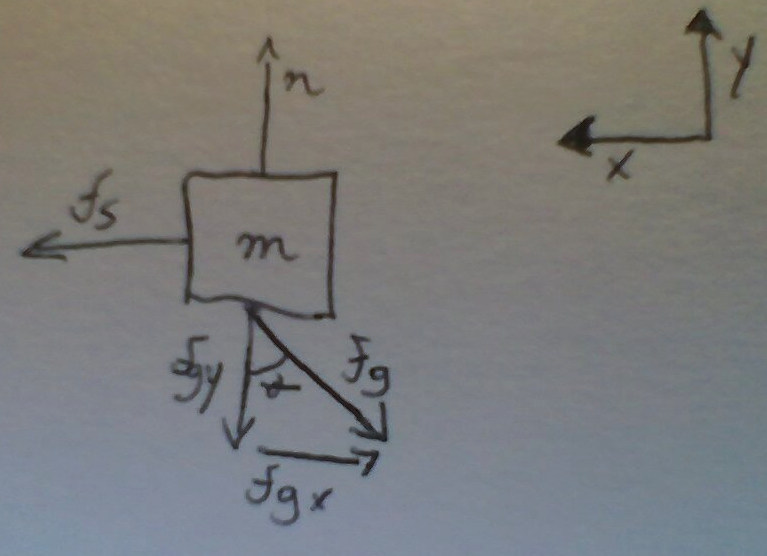
\includegraphics[scale=0.3]{hw6_problemd_fbd}
			\caption{Free-Body Diagram (Problem 13)}
			\label{fig:hw6_problemd_fbd}
		\end{center}
	\end{figure}

	\begin{align}
		f_{s} = \ &f_{s_{max}} = \mu_{s}n = (0.044)n& \notag
	\end{align}

	Newton's $2^{nd}$ Law:
	\begin{align}
		\sum F_{y} = \ &ma_{y}& \notag \\
		n - (mg \cos \theta) = \ &m(0)& \notag \\
		n = \ &mg \cos \theta& \notag \\
		\sum F_{x} = \ &ma_{x}& \notag \\
		f_{s} - (mg \sin \theta) = \ &m(0)& \notag \\
		(0.044)(mg \cos \theta) = \ &mg \sin \theta& \notag \\
		\frac{mg \sin \theta}{mg \cos \theta} = \ &0.044& \notag \\
		\tan \theta = \ &0.044& \notag \\
		\theta = \ &\tan^{-1} 0.044& \notag \\
		= \ &2.52^{o}&
	\end{align}
